\documentclass[tikz, margin=25mm]{standalone}
\usepackage{tikz}
\usetikzlibrary{shapes.geometric, arrows, positioning, decorations.pathreplacing, calc, matrix, fit}
\usepackage[margin=0.5cm]{geometry}


\begin{document}

\begin{tikzpicture}[node distance=2cm and 2cm,
  % every node/.style={inner sep=0,outer sep=0}
  inner/.style={circle,draw=blue!50,fill=blue!20,thick},
  outer/.style={draw=black,fill=gray!10,thick,inner sep=10pt},
  mymatrix/.style={matrix of nodes, nodes=typetag, row sep=1em},
  mycontainer/.style={draw=gray, inner sep=1ex},
  typetag/.style={draw=gray, inner sep=1ex, anchor=west},
  title/.style={draw=none, color=gray, inner sep=0pt},
  ]

  \node[outer, remember picture] (input) {
      \begin{tikzpicture}
  \node[] (mapper) {
      \begin{tikzpicture}
          \foreach \y in {0,1,...,8}
              {
              \node[circle, draw=black, fill=green, minimum size=0.01cm, scale=.3] at (0, -\y*0.5) {};
              \node[circle, draw=black, fill=green, minimum size=0.01cm, scale=.3] at (0.1, -\y*0.5) {};
              \node[circle, draw=black, fill=green, minimum size=0.01cm, scale=.3] at (0.2, -\y*0.5) {};
          }
      \end{tikzpicture}
  };

  %\node[below left=0.0cm and 0.9cm of bottom left, anchor=north west, text width=4.2cm, align=center] (label) {Training data feature-vectors, labelled with a confounding variable };
  \node[below=.0cm of mapper, text width=4.2cm, align=center] (label) {Training data feature-vectors, labelled with a confounding variable };

  \end{tikzpicture}
};


\node[outer, remember picture, right=3cm of input] (lpmodel) {
    \begin{tikzpicture}

      \node[] (lay1) {
        \begin{tikzpicture}
\foreach \y in {0,1,...,8}
    {
        \node[circle, draw=black, fill=green, minimum size=0.01cm, scale=.3] (dot1\y) at (0, -\y*0.5) {};
    }
          \end{tikzpicture}
        };
      \node[right=-0.10cm of lay1] (lay2) {
        
\begin{tikzpicture}
\foreach \y in {0,1,...,2}
    {
        \node[circle, draw=black, fill=green, minimum size=0.01cm, scale=.3] (dot2\y) at (0, -\y*0.5) {};
    }
          \end{tikzpicture}
        };


        \foreach \y in {0,1,...,8}
        {
            \foreach \z in {0,1,...,2}
            {
                \draw[-] (dot1\y) -- (dot2\z);
            }
        }

      % \node [below=.0cm of mapper] (ssl) {Additional layers};

    \end{tikzpicture}
  };

\node[outer, remember picture, right=3cm of lpmodel] (analysis) {
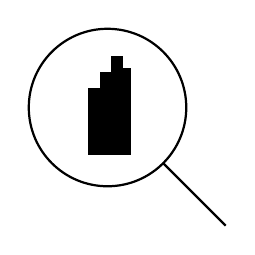
\begin{tikzpicture}
    \draw[thick] (0,0) circle (1cm); % Outer circle
    \draw[thick] (1.5,-1.5) -- (0.7,-0.7); % Handle

    \fill (-0.25,-0.6) rectangle (-0.1,0.25); % First bar
    \fill (-0.1,-0.6) rectangle (0.05,0.45); % Second bar
    \fill ( 0.05,-0.6) rectangle (0.2,0.65); % Third bar
    \fill ( 0.20,-0.6) rectangle (0.3,0.50); % Fourth bar
\end{tikzpicture}
};

\node [above=.0cm of input] (inputText) {1. Organize input};
\node [above=.0cm of lpmodel, text width=3.9cm] (additionalText) {2. Train a linear model};
\node [above=.0cm of analysis, text width=4.2cm] (analysisText) {3. Analyze results, either overall or by class};

\draw[->] (input) -- (lpmodel);
\draw[->] (lpmodel) -- (analysis);

 
\end{tikzpicture}
\end{document}

